\section{Artificial Neural Networks}
\subsection{Introduction}
% Intro
Artificial neural networks have been developed based on the imitation of simplified human neurons, as a framework for function approximation \cite{mcculloch1943logical}. Generally, a neural network is a computational graph whose

\begin{itemize}
  \item Source nodes are numerical inputs or parameters.
  \item Terminal node is the loss function.
  \item Intermediate nodes are operators or functions.
  \item Edges that directly point to the loss function node carry numerical outputs.
\end{itemize}

The shapes of inputs and outputs match the training dataset.

\begin{example}
  \label{example:linear-regression-neural-network}
  Linear regression can be illustrated as a neural network. Take a simple two-dimensional case. Let $((x_1,x_2)_n, \hat{y}_n)_{n=1}^N$ be the dataset and the mathematical model is
  $$y = w_1x_1 + w_2x_2.$$
  The corresponding neural network is shown in Figure \ref{figure:linear-regression-neural-network}.
  \begin{figure}[ht]
    \centering
    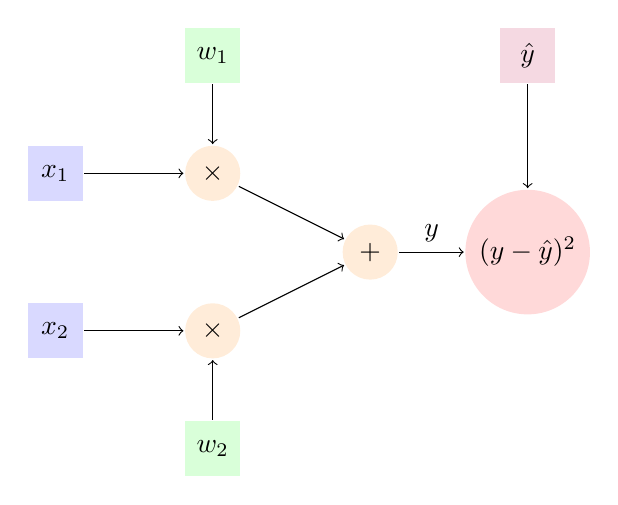
\begin{tikzpicture}[
        inputx/.style={rectangle, fill=blue!15, very thick, minimum size=7mm},
        inputy/.style={rectangle, fill=purple!15, very thick, minimum size=7mm},
        param/.style={rectangle, fill=green!15, very thick, minimum size=7mm},
        function/.style={circle, fill=red!15, very thick, minimum size=7mm},
        operator/.style={circle, fill=orange!15, very thick, minimum size=7mm},
      ]
      %Nodes
      \node[inputx]    (x1)     at (0,0)     {$x_1$};
      \node[inputx]    (x2)     at (0,-2)     {$x_2$};

      \node[param]    (w1)     at (2,1.5)     {$w_1$};
      \node[param]    (w2)     at (2,-3.5)     {$w_2$};

      \node[operator] (times1) at (2,0)     {$\times$};
      \node[operator] (times2) at (2,-2)   {$\times$};

      \node[operator] (add)    at (4,-1)     {$+$};

      \node[inputy] (yhat)    at (6,1.5)     {$\hat{y}$};
      \node[function] (loss)    at (6,-1)     {$(y-\hat{y})^2$};


      %Lines
      \draw[->] (x1) -- (times1);
      \draw[->] (w1) -- (times1);
      \draw[->] (x2) -- (times2);
      \draw[->] (w2) -- (times2);

      \draw[->] (times1) -- (add);
      \draw[->] (times2) -- (add);

      \draw[->] (add) -- node[above] {$y$} (loss);
      \draw[->] (yhat) -- (loss);
    \end{tikzpicture}
    \vspace{0.5cm}
    \caption{The neural network for two-dimensional linear regression}
    \label{figure:linear-regression-neural-network}
  \end{figure}
\end{example}

In Example \ref{example:linear-regression-neural-network}, the output $y$ is just a linear combination of $x_1$ and $x_2$ weighted by $w_1$ and $w_2$. Hence, parameters of a neural network is also called weights. Besides linear combinations, nodes of non-linear functions, called \textit{activation functions}, are added to the neural network for specific tasks. Each instance in the dataset is fed into the neural network. The loss function for linear regression is the norm square. Our objective is to choose parameters $w_1$ and $w_2$ such that the loss function is minimizing over the dataset.

\begin{equation}
  \min\limits_{w_1,w_2} \sum\limits_{n=1}^N (y_n-\hat{y}_n)^2.
\end{equation}

In the next subsections, we discuss the strategy to find the optimal parameters for a neural network.

% Numerical example

\subsection{Optimization Algorithms}

\subsection{Backpropagation}

\subsection{Popular Architectures}




% Element: linear and non-linear

% Example

% Some groundbreaking developments